\documentclass{article}

\usepackage{amsmath}
\usepackage{amssymb}
\usepackage{graphicx}

\begin{document}

\section{Logistic Model and Data}

\subsection{Interpreting the Coefficients}

One of the simplest models of population growth is the logistic equation:

\begin{align}
	\frac{dN}{dt} & = r N (1 - \frac{N}{K})
\end{align}

\subsubsection{Significance of $K$}

The constant $K$ in the model represents the ``carrying capacity'',
	the equilibrium population.
This model (which only makes sense for positive $N$) assumes that there
	is a certain constant, $K$, below which the population will always
	increase, and above which the population will decrease.
The value of $K$ determines at what population $N$ the population
	is in a stable equilibrium.
At that population, $\frac{dN}{dt}$ is zero.

\subsubsection{Significance of $r$}

The constant $r$ in the model represents the speed of population movement.
The value of $r$ doesn't change any of the qualitative aspects of the model.
The time axis of the solution should be interpreted in units of $\frac{1}{r}$.


\subsection{Responding to Data}

To try to evaluate how good this model is, we should compare its
	predictions based on earlier data with the values of later data.
First, we should solve the differential equation.

\subsubsection{Solution and Interpretation of the Differential Equation}

The reader can check that for $r$, $K$ constants, the function below
	satisfies the differential equation in question:

\begin{align}
		N(t) & = K \left( \frac{ A e^{r t}}{1 + A e^{r t}} \right)
\end{align}

The integration constant $A$ is a free parameter which we can use to make
	the line intersect a chosen point.

Suppose we gather a data point that the population is $N_0$ at time $t_0$.
Then, what is $A$?

\[ N(t_0) = K \left( \frac{ A e^{r t_0}}{1 + A e^{r t}} \right) \]

So therefore:

\[ \frac{N_0}{K} = \frac{ A e^{r t_0}}{1 + A e^{r t}} \]

from which we deduce:

\[ A = \frac{N_0}{K - N_0} e^{- r t_0} \]

If we plug this into the original model, we obtain:

\begin{align}
		N(t) & = K \left( \frac{N_0 e^{r(t-t_0)}}{(K - N_0) + N_0 e^{r (t-t_0)}} \right)
\end{align}

Suppose at time $t_1$, the population 


\subsection{d}

\includegraphics[width=0.5\textwidth]{para-pop.png}

The paramecium data seems initially exponential, but then wild fluctuations enter
	in as time goes on later.
These fluctuations seem like complicated, dynamic behavior resulting from interactions
	with the environment.
They may only be explainable by appealing to the spatial distribution of paramecia,
	or modeling something which this model doesn't take into account.
A better model might only claim to fit the initial portion of the data which is exponential.
Or it might use additional data.

\includegraphics[width=0.5\textwidth]{us-pop.png}

The US Census data seems well-fit by an exponential model, or the leading part of a logistic
	model.
It seems like it's trending upwards in a seemingly exponential fashion.
An exponential model might explain the data more simply in this case.


\section{Marriage age}

\subsection{Differential Equation for Marriage}

Assume the following factors affect a person's likelihood of
	marrying in a time interval $\Delta t$:

\begin{enumerate}
	\item The likelihood is proportional to the length of 
			the time interval $\Delta t$
	\item The likelihood is proportional to the fraction of 
			people in the person's age group
			who are already married, $m(t)$.
\end{enumerate}

\subsubsection{Derivation of Differential Equation}

Suppose there are $N$ people.
The likelihood that one individual marries is proportional to
	$\Delta t m(t)$, based on the above assumptions.
Since there are $N (1 - m(t))$ unmarried people, in a large enough
	sample size the expected number of marriages in a time interval
	$\Delta t$ is $N (\Delta t) m(t) (1 - m(t))$
Therefore, the fraction of people married in a time interval $\Delta t$,
	which I will denote $\Delta m$, is proportional to 
	$(\Delta t) m(t) (1 - m(t))$.
Taking the limit of difference quotients, we arrive at the following
	differential equation:

\begin{align}
		\frac{dm}{dt} & = c m(t) \left( 1 - m(t) \right)
\end{align}

where $c$ is a constant of proportionality.

\subsubsection{Solution of Differential Equation}

We begin with:

\[ \frac{dm}{dt} = c m (1-m) \]

We first split the derivative into two differntials and bring them
	to opposite sides:

\[ \frac{dm}{m(1-m)} = c dt \]

We want to integrate these two differentials.
We should express the left hand side in terms of a sum of two fractions.

Suppose, for unknown $A$ and $B$, the following equation is an identity:

\[ \frac{A}{m} + \frac{B}{1-m} = \frac{1}{m(1-m)} \]

Then by multiplying, the following equation should be an identity for all $m$.

\[ A(1-m) + B m = 1 \]

Specifically, for $m$= 1, we deduce:

\[ B = 1 \]

And for $m = 0$, we deduce:

\[ A = 1 \]

Huh.  We probably should have guessed.  Oh well.

Anyways, the differential equation can now be written:

\[ \frac{dm}{m} + \frac{dm}{1-m} = c dt \]

Integrating these seperately, we obtain:

\[ log(m) - log(1-m) = c T  + C\]

Taking the exponential of both sides, we obtain:

\[ \frac{m}{1-m} = \exp{c T}\exp{C} \]

For convenience, we define $A = \exp{C}$ to be a positive number.

This equation implies:

\[ m = (1 - m) A \exp{c T} \]

We then bring the $m$'s over to the left side:

\[ m ( 1 + A \exp{c T} ) = A \exp{c T} \]

Finally, we achieve an expression for $m(t)$:

\begin{align}
	m(t) & = \frac{A e^{c T}}{1 + A e^{c T}}
\end{align}



\subsection{Criticism of the Model}

This model is extremely simplistic and only attempts to capture
	peer behavior.
Notably, the model completely ignores age.
It assumes that everybody has the same peer group, and are equally
	influenced by every pressure.
However, the model does capture the central characteristics of marriage
	based on peer influence, which are widely observed and documented.
The model may have a limited range of applicability:
	perhaps the model becomes effective among a certain population,
	for example people between the ages of 25 and 35 with relatively
	large social circles.
Group pressure may influence these people to formalize their relationships.
However, the model will not be effective when there are comparatively few
	marriages.
When there are many marriages at once, though, the model predicts that
	their distribution may look somewhat like the logistic curve.

\subsection{Time-varying Proportionality Constant}

Suppose the constant of proportionality $c$ is changing in time.
The first thing we should do is add an additional assumption:

\begin{enumerate}
	\setcounter{enumi}{2}
	\item The likelihood of an individual marrying is proportional to
			a function of time $c(t)$.
\end{enumerate}

\subsubsection{Discussion of the Significance of the Time-Varying Constant}

The time-varying constant can help the model by speeding up or slowing down 
	the rates of marriage at certain times.
For example, if the model is applied to a localized age cohort, 
	the function $c(t)$ could be proportional to salaries wihin the age cohort,
	or otherwise somehow related to external factors which may cause marriage.
It would be an interesting population-modeling result to fit marriage rates
	within a social cohort to, for example, a logistic model with $c(t)$ 
	proportional to mean standard of living within the cohort.
This would be a quantitative way of saying that the two most significant factors
	which influenced marriage within this age cohort are standard of living and
	peer pressure.

\subsubsection{Solution the Time-Varying Constant in the Differential Equation}

We repeat the analysis above, but with one change.

Above, we integrated

\[ c dt \]

to obtain

\[ c T + C \]

Here, if $c = c(t)$, we integrate

\[ c(t) dt \]

to obtain

\[ \int_0^t c(t) dt + c(0) \]

If we repeat the rest of the analysis, the overall solution becomes:

\begin{align}
	m(t) & = \frac{A e^{\int_0^t c(t) dt}}{1 + A e^{\int_0^t c(t)}}
\end{align}

\subsubsection{Predicting Marriage Fractions in my Age Class}

I might observe in popular culture that the standard ages for marriage
	are between $25$ and $40$.
I propose the following $c(t)$:

\[ c(t) = \left\{ 
	\begin{array}{cc} 
			0 & 0 \leq t \leq 25 \\ 
			0.04 & 25 < t \leq 40 \\
			0 & 40 < t
	\end{array} \right\} \]

Some small fraction $m_0$ of people are married at $25$.
To find out $A$ from this, we note:

\[ m(0) = \frac{A}{1 + A} \]

And from this we deduce:

\[ A = \frac{1}{1 - m_0} \]

Suppose $5$ percent of people are married at age $25$.
Then, $A \approx 1.05$

Therefore, by the time $t = 40$,

\[ m(40) = \frac{A e^{0.04 * 25}}{1 + A e^{0.04 * 25}} \approx 0.74
\]

This prediction is contingent on choice of $c$ and assumption that 5
	percent of people marry by 25.

\subsection{Properties of a good $c(t)$}

A good $c(t)$ will explain several observations:

\begin{enumerate}
	\item Nobody marries before the age of 18.
	\item Very few people marry before the age of 23.
	\item Marriages seem to peak between late twenties
		and late thirties.
	\item There are very few marriages after the forties.
\end{enumerate}

The $c(t)$ should therefore be zero for $t \leq 18$,
	increase slowly until it reaches its peak in the mid
	thirties, and then decrease until it is near zero
	in the late forties.

\subsection{Initial Conditions}

Since $m(t)$ was zero at age 18, naively the model predicts
	no marriages.
However, this shouldn't be taken seriously.
The model is only applicable when there are enough marriages
	in a population for there to be significant peer pressure
	to marry.
Therefore, we should choose a small value of $m$ and declare
	that the model doesn't apply below it, that other
	factors predominantly influence marriage rates.
Then, once those other factors predict the marriages to rise
	significantly, we should start using our logistic model.

\subsection{Modeling Differences in Personality}

Can we use this model to describe a certain fraction of the population
	who does not want to marry?
We cannot, because as long as the integral of $c(t)$ increases,
	which it will as long as $c$ is postive,
	the marriage fraction will increase to 1.
Therefore, we should treat $m$ as the fraction of marriagable people
	who are married.

Can we use this model to describe a range of preferences in what ages
	people want to marry at?
If instead of being sharply peaked, $c(t)$ is nonzero over a long range,
	this seems to capture this behavior.
The marriage fraction will be steadily but slowly increasing as more people
	reach the different ages at which they want to marry.

\subsection{Transformation of the Axis}

Some statisticians found that if we make a linear transformation of the age axis
	and a scale transformation of the proportion married axis,

\[ y = e^{-e^{-x}} \]

fits the data very closely.

This fits in with the previous discussion because the fraction married
	exponentially approaches the measured fraction at infinity.
I don't see any motivation for this model, however.

i

\section{ Stochastic Modeling of Logistic Model }



\subsection{Gossip Propagation}

I want to make a stochastic model to model gossip propagation.
Gossip starts as something that $N_0$ people know,
	where $N_0$ is a positive integer between $0$ and
	$K$ (representing the total population size).
We want a rule to stochastically update a variable $N$, which
	represents the number of people who know the gossip,
	in discrete time steps.
We make the following assumptions:

\begin{enumerate}
\item Nobody ever forgets the knowledge, 
	so $N$ never decreases.
\item People who do not know the gossip must learn it from
	somebody who does.
\item Everybody has an equal chance of meeting everybody
	else each round.
Nobody meets themself.
\item There are an even number of people, so everybody
	is in exactly one two-person meeting per round.
\item During a meeting, every person who knows the information
	reveals it to the other person.
\end{enumerate}

Each time step, each member of the population will meet a
	single other member of the population.
The only meetings which spread gossip are meetings between
	people who know the gossip and people who do not.
If there are $K$ total people and $N$ know, we ask what
	is the probability of exactly $a$ meetings between
	knowledgables and ignorants?
This probability will be equal to the number of ways that $a$
	meetings between $N$ knowledgables and $K-N$ ignorants
	can occur, divided by the total number of possible 
	pairings.

\subsection{Total Number of Pairings in $K$ people}
How many ways $p_K$ are there for $K$ people to arrange themselves
	into pairs?
There is no way if $K$ is odd, so let us assume $K$ is even.

If we first divide $K$ people into pairs, order the pairs,
	and order the individuals in each pair,
	we have ordered $K$ individuals.
There are $K!$ ways of ordering $K$ individuals,
	and since there are $K/2$ pairs there are
	$(K/2)!$ ways of ordering the pairs.
Since there are $2$ orders each pair can be in, 
	and $K/2$ pairs, there are $2^{K/2}$
	possible orderings of the individuals within the pair.
Therefore:

\[ p_K (K/2)! 2^{K/2} = K! \]

or equivalently:

\begin{align}
p_K & = \frac{K!}{(K/2)! 2^{K/2}}
\end{align}

\subsection{Total number of ways to form $a$ pairs
	with one individual one of $N$ individuals and 
	the other individual one of $K-N$ individuals}

We need to find out how many ways there are to form $a$
	pairs between the $N$ knowledgeables and the $K-N$
	ignorants.

Before we begin, let's note that if there are an even number
	of knowledgables, there is no way that $a$ can be
	odd because one knowledgable would be unpaired.
Similarly, if there is an odd number of knowledgables
	there can't be an even number of pairs.

Let's select $a$ knowledgables
	and $a$ ignorants.
Since the two are chosen independently, the total number 
	of ways of doing this is:

\[ { N \choose a} {K - N \choose a} \]

We now have to choose which knowledgeables match with which
	ignoramuses.
We can arbitrarily label the $a$ knowledgeables, and then
	the number of possible matchings will be the number
	of ways of ordering $a$ elements, which is $a!$.
The total number of ways of pairing up $N$ knowledgables
	with $N-K$ ignoramuses is thus:

\[ {N \choose a} {K -N \choose a} a! \]

But wait, there's more!
We still need to pair up the unpicked knowledgeables and 
	ignoramuses with each other.
Fortunately we have done this calculation already.
Since there are $N-a$ unpaired knowledgables
	and $K-N-a$ unpaired ignoramuses,
	and they are paired independently,
	the total number of ways of pairing them together 
	will be the product of the number of ways 
	of pairing them off individually.
The total number of ways of pairing all $K$ individuals,
	with exactly  $a$ connections between $N$
	knowledgables and $K-N$ ignoramuses is thus:

\begin{align}
n_{N,K,a} & = \frac{(N-a)!}{2^{(N-a)/2} ((N-a)/2)!}
	{N \choose a}
	a !
	{K - N \choose a}
	\frac{(K - N - a)!}{2^{\frac{K - N - a}{2}} 
		(\frac{K-N-a}{2})!}
\end{align}

\subsection{Turning $n_{N,K,a}$ into a normalized probability
	there there are $a$ connections}

To turn (2) into a probability that there are $a$ connections,
	we need to divide by the total number of configurations.
We have already computed this, it is (1).
After much algebra, the normalized form becomes:

\begin{align}
p_{N,K,a} & = \frac{(K/2)!}{{K \choose N}}
	\frac{2^a}{ \left(\frac{N - a}{2}\right)!
		\left(\frac{K - N - a}{2}\right)!
		a! }
\end{align}

Since only some of this depends on $a$, we can search for
	a recurrence relation to simplify computation.
After more algebra and separation, I find:

\begin{align}
p_{N,K,a+2} & = \frac{(N - a)(K - N - a)}{(a + 1)(a + 2)} 
	p_{N,K,a}
\end{align}

Note that the numerator means that it is not possible to form
	more than $N$ or $K-N$ connections.

\subsection{Implementation of a Stochastic Model}

To implement a stochastic model based on these probabilities,
	I need to choose an even $K$ and a starting population
	$N_0$.
Then each round, I create a probability distribution over the
	different values of $a$ and sample from it.
The $a$ ignoramuses who were selected now become knowledgables,
	so $N$ is incremented by $a$.
The process then repeats.

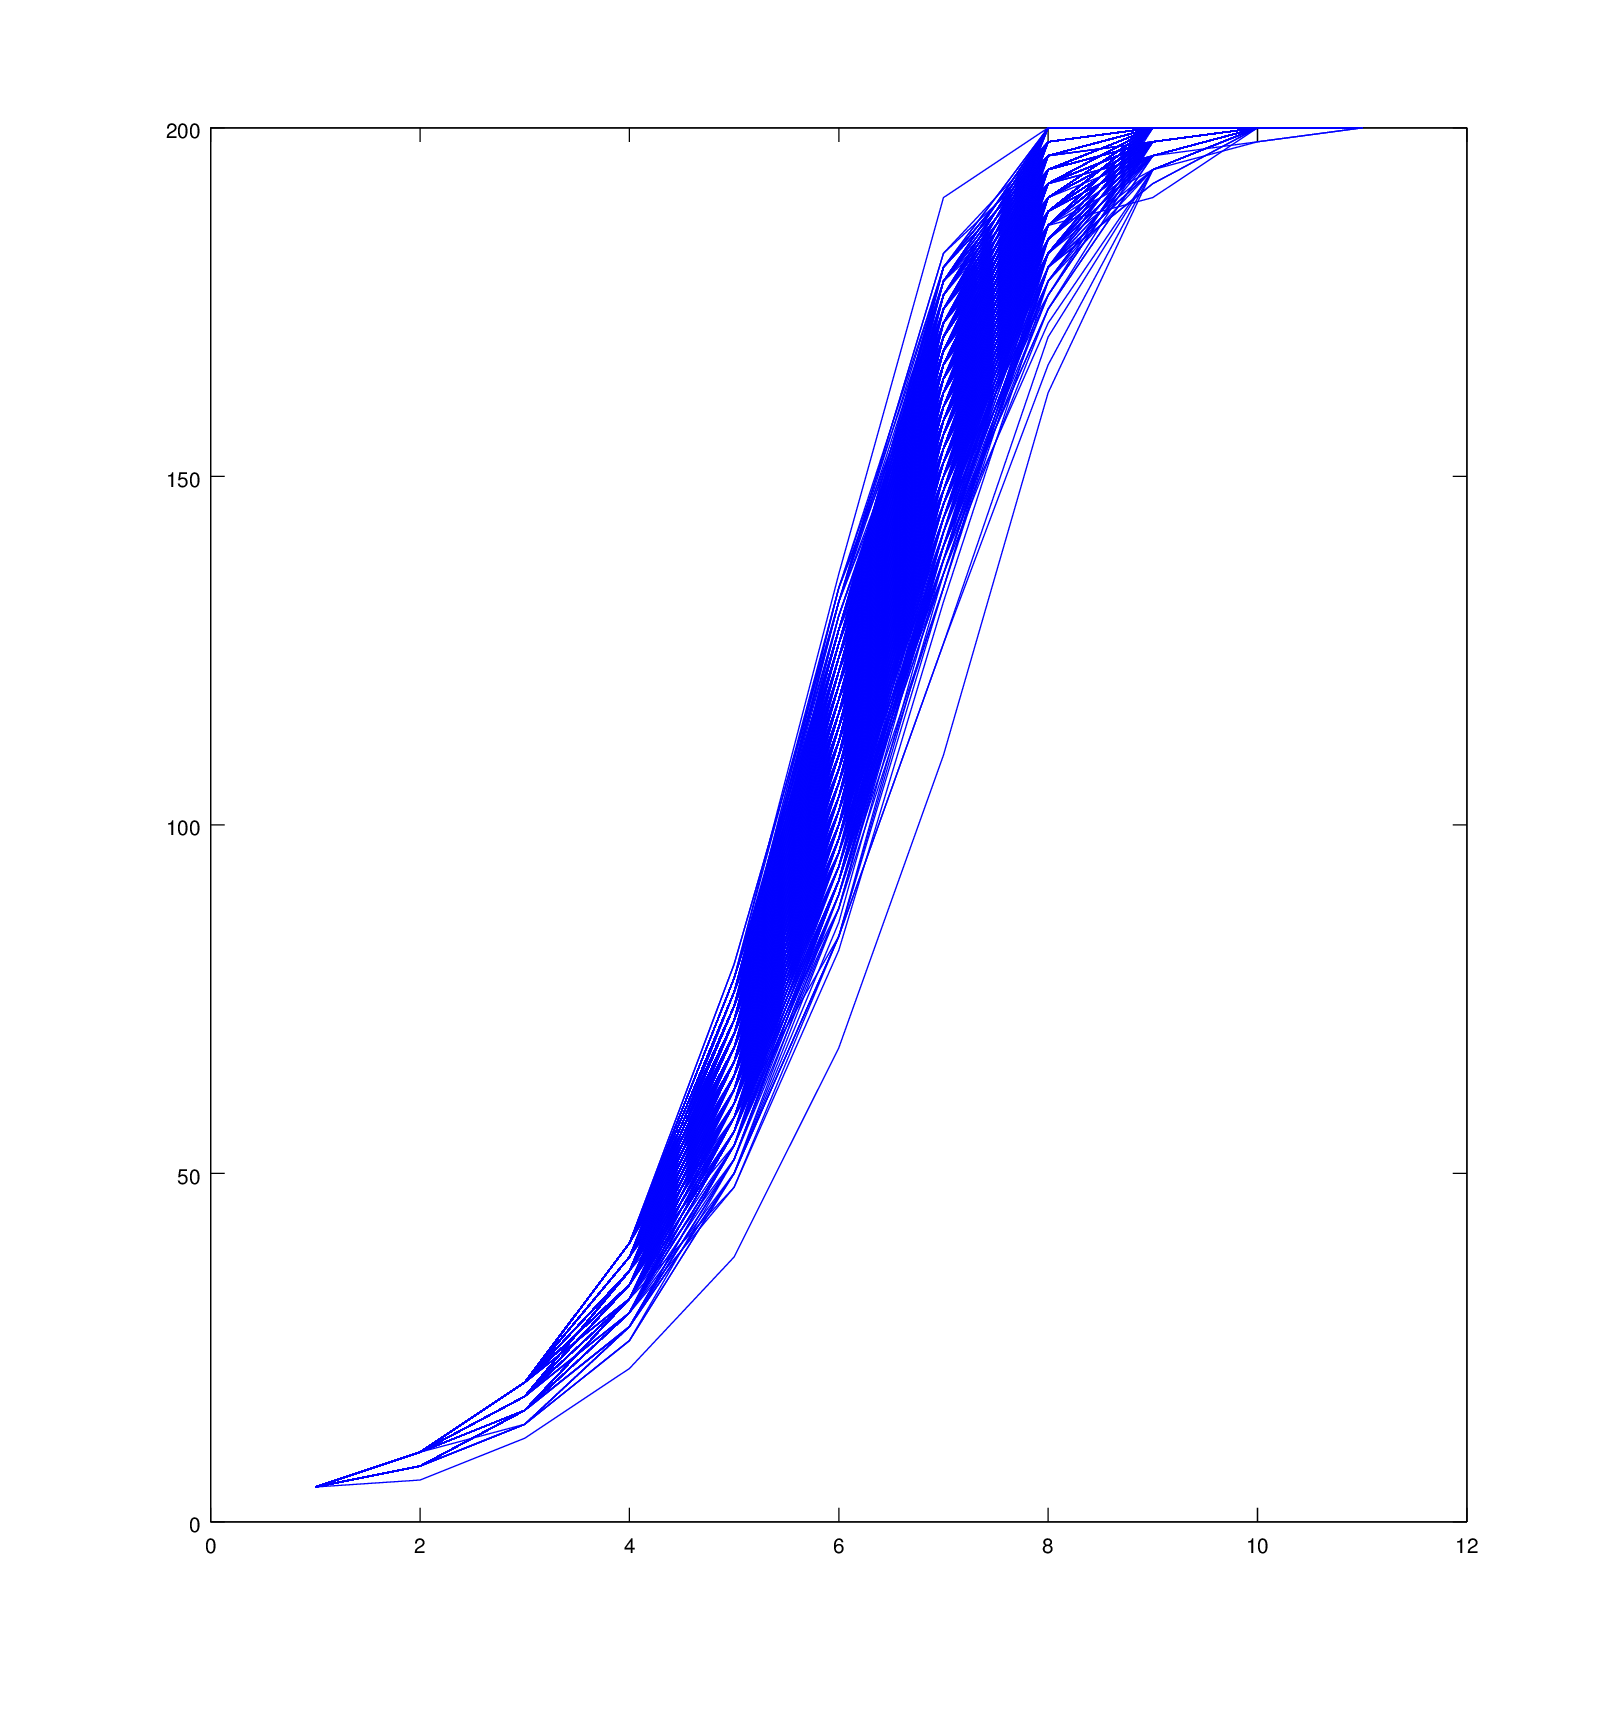
\includegraphics[width=0.7\textwidth]{lines.png}

This is a stochastic model.

\subsection{Extension to coefficients $c$}

In order to have more parameters, we could introduce a parameter $c$
	which represents the probability that two people who meet
	decide to share their knowledge.
Since we have determined the probability that $a$ people meet,
	we can sample that distribution and then find out how many
	meetings there are beween knowledgables and ignoramuses.
Then we can sample from a binomial distribution in $c$ ranging from $0$ to $a$
	to get the expected number of ignoramuses converted into knowledgables.

\section{Stochastic Modeling of Population Growth}

\subsection{Asexual Reproduction with Predation}

Consider a species of creature which reproduces asexually, and fights one another.
The probability of two such creatures coming close enough together to begin a life-or-death
	struggle is proportional to the square of the population,
	so the change in population is weighted downwards by $N^2$, where $N$ is population.
Also, each creature reproduces independently, so the change in population is weighted 
	upwards by $N$.

Suppose each round, any creature has a chance $p$ of meeting any other in a life-or-death struggle.
Then, each creature has a probability of $(N-1)p$ of engaging in a life-or-death struggle.
The probability of $n$ life-or-death struggles is thus a binomial distribution on $(N-1)p$.



\subsection{Sexual Reproduction}

To model population growth, we can re-use a significant portion of the previous analysis.
Suppose we have a population of $N$ members, with $N_m$ males and $N_f$ females.
Each round, every member of the population randomly meets another.
Then, at the end of the round, natality and mortality happen.
For every meeting between creatures of the opposite sex,
	there is a probability $p$ of the female becoming pregnant.
The next round, the female will give birth to a creature which is equally likely
	to be male or female.

For each meeting between males, there is a probability $f$ that they will fight.
If they fight, then one of them will die.
Since we already determined the number of male-female meetings, the number of male-male
	meetings is the $\frac{N_m - N_{\text{meetings}}}{2}$.
Therefore, each round, the male population goes down by a number drawn from a binomial 
	distribution with probability $f$ from $0$ to $\frac{N_m - N_{\text{meetings}}}{2}$.

At the same time, there is a death rate $d$.
Each round, every creature might die with probability $d$.
Since the births take place at the end of the round, we should compute deaths
	before births.

To update the numbers $N_m$ and $N_f$ for each round, we need to compute the following:

\begin{enumerate}
\item Begin with $N_m$ males and $N_m$ females.
\item Determine the number of meetings between creatures of the opposite sex.
	As discussed before, the normalized probability of $a$ meetings is:
	\[ M_{N_m, N_f, a} = \frac{ \left( \frac{N_m + N_f}{2} \right)!}{ { N_m + N_f \choose N_m}}
					\frac{ 2^a } { \left( \frac{N_m - a }{2} \right)!
									\left( \frac{N_f - a}{2} \right)!
					a! } \]
		if $N_f + N_m$ is even.
	If it isn't, we randomly choose an "odd one out" from either sex,
		and then compute.
	First, we should obtain the total number of meetings, $M$, by sampling the distribution.
	
\item Next, we should sample from a binomial distribution on $M$ letters with probability $p$,
		to get the number of pregnancies $N_p$.
\item Then, we should sample from a binomial distribution on $floor((N_m - M)/2)$ letters
		with probability $f$ to get the number of males dead from fighting, $D_g$.
\item Sample from a binomial distribution of $N_m$ elements with probability $d$,
		to obtain the $D_m$, the number of dead males from natural causes.
	Similarly obtain $D_{nf}$, the number of dead females who are not pregnant,
		and $D_{pf}$, the number of dead pregnant females.
\item Finally we need to determine the number of births of each sex.
		The total number of male babies and of female babies is determined by sampling
			a binomial distribution on $N_p - D_{pf}$ with even probability.
		This gives us a number of male babies $B_m$, and a number of female babies $B_f$
\item Update the populations:
		\begin{align*}
				N_m(t+1) & = N_m(t) - D_m - D_g + B_m \\
				N_f(t+1) & = N_f(t) - D_{nf} - D_{pf} + B_f \\
		\end{align*}
\end{enumerate}
\end{document}
